\section{Descripción de los juegos}
\label{section-description-juegos-forma-extensiva}

Para probar los algoritmos se implementaron tres tipos de juegos diferentes: \textit{One Card Poker} (OCP), \textit{Dudo}, un juego de dados, y una versión del juego de dominó para $2$ personas. La descripción detallada de las reglas de los juegos se describen en esta sección.

\subsection{One-Card Poker}
One-Card Poker, abreviado OCP(N), es la versión generalizada del juego Kuhn Póker, explicado en la sección \ref{section:kuhn-poker}. En este juego, cada jugador recibe una carta de un mazo de $N$ cartas, y luego pueden apostar o retirarse según las mismas reglas del Kuhn Póker. Note que OCP(3) es equivalente al Kuhn Poker. El árbol de este juego tiene $9N(N-1)+1$ nodos (incluyendo el nodo inicial, que es el nodo de azar) y hay $4N$ conjuntos de información entre ambos jugadores. 

\subsection{Dudo}
Dudo, también conocido como \textit{Bluff}, \textit{Liar's Dice} o Perudo, es un juego de dados y apuestas. Usualmente se juega entre $2$ y $6$ jugadores. Los jugadores se ubican en forma circular y cada uno de ellos tiene un número de dados. De forma simultánea, todos lanzan sus dados, cada jugador puede ver el resultado de sus propios dados, pero no puede ver el resultado de los dados de los otros jugadores. Una vez hecho esto, los jugadores empiezan a apostar sobre el número de veces que apareció una cara en específico en todos los dados que hay en la mesa.

Una apuesta consiste en decir $2$ números $(x, y)$, esto indica que el jugador apuesta que hay, al menos, $x$ dados cuyo resultado fue el número $y$. El primer jugador (que se elige previamente mediante el lanzamiento de $1$ dado o de alguna otra forma), realiza la primera apuesta y, en sentido horario, cada jugador puede hacer una apuesta más alta o decir \say{dudo} y retar al jugador anterior. Una apuesta es más alta que otra si el número de dados que se anuncian en la apuesta ($x$) es mayor, o si el número de dados es igual, pero la cara apostada ($y$) es mayor. Por ejemplo $(3, 1)$ es mayor que $(2, 5)$, y ambas apuestas son mayores que $(2, 3)$.

Por otra parte, si un jugador reta al jugador previo, se descubren todos los dados de todos los jugadores. Si la cantidad de dados con la cara $y$ es mayor o igual a $x$, donde $(x, y)$ fue la apuesta realizada por el jugador, el jugador que hizo el reto pierde un dado. En caso contrario, el jugador que hizo la apuesta pierde un dado. Luego, todos los jugadores lanzan sus dados nuevamente y una nueva ronda de apuestas empieza por el jugador que perdió la ronda anterior. Un jugador pierde cuando se queda sin dados, el ganador es el último jugador con al menos un dado restante. La figura \ref{fig:dudo} muestra una foto del juego, de \textit{Perudo}, una versión comercial de este juego, que está diseñada para $6$ jugadores, donde cada jugador empieza con $5$ dados. En la figura se observan los vasos que se utilizan para lanzar los dados y evitar que cada jugador vea los dados de los demás.

\begin{figure}[htb]
\caption[Juego Dudo]{Juego Dudo. Los vasos se utilizan para lanzar los dados y evitar que los oponentes vean el resultado}
\label{fig:dudo}
\centering
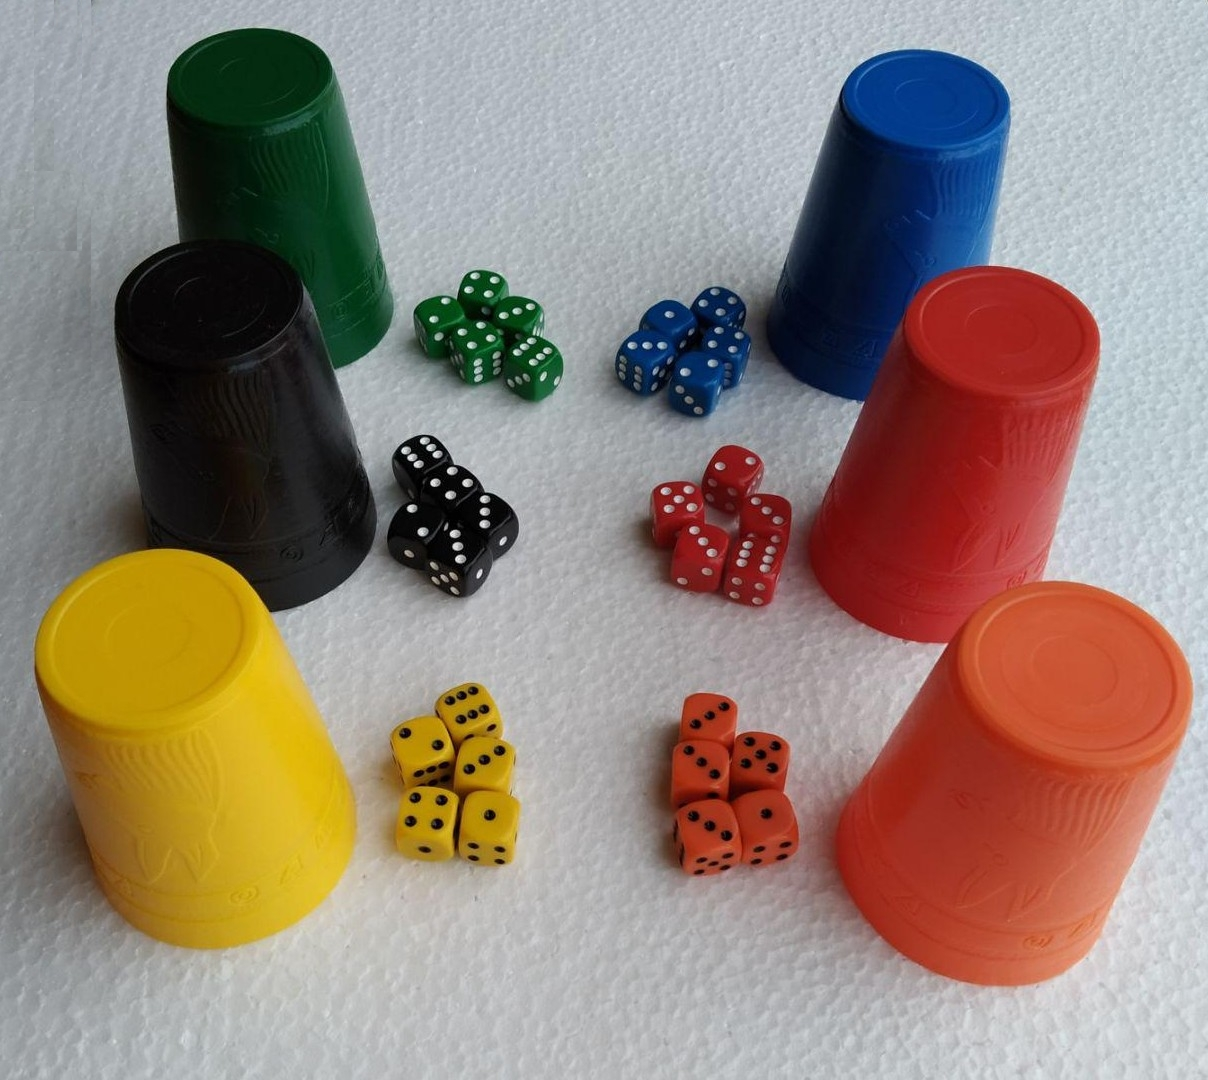
\includegraphics[width=0.6\textwidth]{figuras/dudo.jpg}
\end{figure}

En este trabajo de grado consideraremos este juego para $2$ jugadores únicamente. Dudo$(K, D_1, D_2)$ hará referencia a una única ronda de apuestas de $2$ jugadores, donde el primer jugador tiene $D_1$ dados, el segundo jugador tiene $D_2$ dados y cada dado tiene $K$ caras. El juego completo consiste en múltiples rondas, donde $D_1$ o $D_2$ disminuye en una unidad al finalizar cada ronda. Cuando uno de los jugadores pierde todos los dados obtiene una utilidad de $-1$, mientras que su oponente obtiene una utilidad de $1$. En este juego cada ronda se considerará un subjuego y se representará con un árbol independiente, donde los valores esperados para los juegos Dudo$(K, D_1 - 1, D_2)$ y Dudo$(K, D_1, D_2 - 1)$ se precalculan y se utilizan como utilidad para las hojas del árbol Dudo$(K, D_1, D_2)$. Note que, en el juego estándar, $K$ siempre tiene un valor de $6$.

Cuando el jugador $i$ lanza $D_i$ dados hay $\binom{D_i+K-1}{K-1}$ resultados posibles diferentes, ya que cada resultado puede ser representado con una tupla $(a_1, a_2, ..., a_k)$, donde $a_j$ representa el número de dados con la cara $j$, por lo que $\sum_j^K = D_i$ y $a_j \geq 0$. Por otra parte cada secuencia de apuestas puede ser representada por una secuencia binaria de longitud $K(D_1 + D_2)$, donde el $i$-ésimo bit es $1$ si la $i$-ésima secuancia más fuerte fue dicha durante la ronda y $0$ en caso contrario. Por ejemplo, si $D_1 = D_2 = 1$, las apuestas $(1, 1)-(1, 3)-(1, 6)-(2, 4)-(2, 5)-(1, 6)$ se representa con la secuencia binaria $101001000110$, por lo que hay $2^{K(D_1 + D_2)}$ secuencias diferentes. Cada secuencia pertenece a un jugador en específico, por lo que si $D_1 = D_2$, el número de conjuntos de información  es igual a  $\binom{D_i+K-1}{K-1}2^{K(D_1 + D_2)}$.

Para contar el número total de nodos, se puede considerar el lanzamiento de los dados de forma independiente, pues las secuencias posibles de apuestas no dependen del resultado de los dados. Por lo expuesto anteriormente el número posible de apuestas es igual a $2^{K(D_1+D_2)}$, pero después de cada secuencia siempre se puede decir \say{dudo}, salvo para la secuencia vacía. Luego el número total de nodos (incluyendo nodos terminales y no terminales) es igual a $\binom{D_1+K-1}{K-1}\binom{D_1+K-1}{K-1}(2^{K(D_1+D_2)+1}-1)+1$.

\subsection{Domino}
En este trabajo se utilizó una versión de este juego para $2$ jugadores. Al inicio del juego cada jugador toma una cantidad específica de piezas de forma aleatoria, las piezas restantes se dejan sin descubrir para ser usadas en turnos posteriores. Como en el juego tradicional de dominó, los jugadores juegan por turnos alternados (el primero jugador se elige de forma arbitraria), cada uno debe colocar una ficha válida acorde a las reglas \textit{estándares} en Venezuela del juego (ver apéndice \textit{\textbf{X}}). Si un jugador no puede colocar una ficha toma una ficha de las que no están descubiertas (si todavía hay disponibles), el jugador verifica si puede colocar la ficha tomada y en caso contrario pasa el turno y juega el oponente.

El juego termina cuando alguno de los jugadores usa todas las piezas o cuando ambos jugadores no pueden jugar ni tomar piezas nuevas, en este último caso se dice que el juego está bloqueado. El ganador es el jugador que se queda sin piezas o, en caso de bloqueo, el jugador que acumule menos puntos en todas las piezas que quedaron en su mano. La utilidad obtenida es el número de puntos que el jugador perdedor acumuló en las piezas que quedaron en su mano (con signo positivo para el jugador ganador y signo negativo para el perdedor). Cabe destacar que sólo se puede tomar una pieza o pasar, si no se puede realizar una jugada con la mano actual.

Usualmente se utilizan $28$ piezas, donde las piezas pueden tener entre $0$ y $6$ puntos en cada extremo, y cada jugador recibe $7$ piezas al inicio del juego. En este trabajo se parametriza el número máximo de puntos que puede tener una ficha, así como la cantidad de piezas repartidas inicialmente. De esta forma se hará referencia a Domino$(M, N)$ an un juego donde las piezas tienen entre $0$ y $M$ puntos (con un total de $M(M+1)/2$ piezas) y cada jugador recibe $N$ piezas al inicio del juego.

En este juego no es fácil calcular el tamaño del árbol y el número de conjuntos de información, principalmente porque las acciones posibles en un estados dependen tanto de la mano del jugador, como de las piezas en la mesa. En el Kuhn Póker simpre hay $2$ acciones posibles ${pasar, apostar}$ y en el Dudo las acciones disponibles dependen únicamente de la última apuesta y no dependen de los dados que tengan los jugadores. Así que se decidió estimar estos parámetros recorriendo el árbol del juego mediante DFS. La tabla \ref{tab:tree-domino}, muestra el número de nodos del árbol y el número de conjuntos de información por cada juego de dominó que se presenta.

\begin{table}[ht]
    \centering
    \begin{tabular}{c|r|r}
        & Conjutos de Información & Nodos \\ \hline
       Domino$(1, 1)$ & $3$ & $13$ \\
       Domino$(2, 2)$ & $441$   & $7321$ \\
       Domino$(3, 2)$ & $844437$   & $46534657$ \\
       Domino$(3, 3)$ & $1082290$   & $246760993$ \\ 
       Domino$(3, 4)$ & $902218$   & $1547645185$ \\ \hline
    \end{tabular}
    \caption{Número de nodos y conjuntos de Información en diferentes juegos de Dominó}
    \label{tab:tree-domino}
\end{table}


